%%%% ijcai21.tex

\typeout{IJCAI--21 Instructions for Authors}

% These are the instructions for authors for IJCAI-21.

\documentclass{article}
\pdfpagewidth=8.5in
\pdfpageheight=11in
% The file ijcai21.sty is NOT the same than previous years'
\usepackage{ijcai21}

% Use the postscript times font!
\usepackage{times}
\usepackage{soul}
\usepackage{url}
\usepackage[hidelinks]{hyperref}
\usepackage[utf8]{inputenc}
\usepackage[small]{caption}
\usepackage{graphicx}
\usepackage{amsmath}
\usepackage{amsthm}
\usepackage{booktabs}
\usepackage{algorithm}
\usepackage{algorithmic}
\urlstyle{same}

% the following package is optional:
%\usepackage{latexsym}
\usepackage{multirow}
\usepackage{makecell}

% See https://www.overleaf.com/learn/latex/theorems_and_proofs
% for a nice explanation of how to define new theorems, but keep
% in mind that the amsthm package is already included in this
% template and that you must *not* alter the styling.
\newtheorem{example}{Example}
\newtheorem{theorem}{Theorem}

% Following comment is from ijcai97-submit.tex:
% The preparation of these files was supported by Schlumberger Palo Alto
% Research, AT\&T Bell Laboratories, and Morgan Kaufmann Publishers.
% Shirley Jowell, of Morgan Kaufmann Publishers, and Peter F.
% Patel-Schneider, of AT\&T Bell Laboratories collaborated on their
% preparation.

% These instructions can be modified and used in other conferences as long
% as credit to the authors and supporting agencies is retained, this notice
% is not changed, and further modification or reuse is not restricted.
% Neither Shirley Jowell nor Peter F. Patel-Schneider can be listed as
% contacts for providing assistance without their prior permission.

% To use for other conferences, change references to files and the
% conference appropriate and use other authors, contacts, publishers, and
% organizations.
% Also change the deadline and address for returning papers and the length and
% page charge instructions.
% Put where the files are available in the appropriate places.

%PDF Info Is REQUIRED.
\pdfinfo{
/TemplateVersion (IJCAI.2021.0)
}

\title{Learning Deeply Enriched Representations of Temporal Data of COVID-19 Patients for Improved Mortality Prediction}

% Single author syntax
\author{
    Anonymous Authors
}

% Multiple author syntax (remove the single-author syntax above and the \iffalse ... \fi here)
% Check the ijcai21-multiauthor.tex file for detailed instructions
\iffalse
\author{
First Author$^1$
\and
Second Author$^2$\and
Third Author$^{2,3}$\And
Fourth Author$^4$
\affiliations
$^1$First Affiliation\\
$^2$Second Affiliation\\
$^3$Third Affiliation\\
$^4$Fourth Affiliation
\emails
\{first, second\}@example.com,
third@other.example.com,
fourth@example.com
}
\fi

\begin{document}

\maketitle

\begin{abstract}
    \iffalse
    Learning compressed representations of multivariate time series (MTS) facilitates data analysis in the presence of noise and redundant information, and for a large number of variates and time steps. However, classical dimensionality reduction approaches are designed for vectorial data and cannot deal explicitly with missing values. In this work, we propose a novel autoencoder architecture based on recurrent neural networks to generate compressed representations of MTS.
    
    Although semi-supervised variational autoencoder (SemiVAE) works in image classification task, it fails in text classification task if using vanilla LSTM as its decoder. From a perspective of reinforcement learning, it is verified that the decoder’s capability to distinguish between different categorical labels is essential. Therefore, Semi-supervised Sequential Variational Autoencoder (SSVAE) is proposed, which increases the capability by feeding label into its decoder RNN at each time-step. Two specific decoder structures are investigated and both of them are verified to be effective.
    \fi
    % The abstract should briefly summarize the contents of the paper in 15--250 words. 
    An influx of Coronavirus Disease 19 (COVID-19) infections puts pressure on healthcare systems and disrupts their general care routine, and efficient allocation of finite resources becomes a crucial problem. To aid logistical decision-making, we propose a novel semi-supervised learning framework to predict clinical outcomes of COVID-19 patients. Because the clinical measurements of COVID-19 patients can be collected over time, our model aims to predict the clinical outcomes from the multivariate time series (MTS) which may contain missing data. We leverage Long Short Term Memory (LSTM) architecture to learn the vectorial representation of MTS with missing data and uneven time intervals between records. Armed with the vectorial representation of MTS, conventional machine learning models can be used to predict the clinical outcomes. In our experiments, the proposed model predicts mortality of COVID-19 patient with the blood samples collected from the 358 patients infected with COVID-19 in Wuhan, China. Our embedding framework shows 88\% to 94\% prediction accuracy, even if very few samples are labeled. In addition, we identify the mortality relevant biomarkers from the proposed method.\footnote{The codes used in our experiments will be made publicly accessible on GitHub upon paper acceptance.}
    %% begin-IB
    % An influx of COVID-19 infections puts pressure on healthcare systems and
    % disrupts their general care routine, leading to an increase in excess
    % deaths. Efficient allocation of finite resources, is a persistent problem
    % most apparent during a sudden influx of patients. Earlier studies have
    % suggested the use of biomarkers, particularly those measured in blood
    % samples, to build mortality-prediction models to aid in logistical
    % decision-making. These same studies focused on isolating predictive
    % biomarkers rather than building a deterministic model. This paper uses
    % longitudinal data collected from blood samples of 375 patients infected
    % with COVID-19 in Wuhan, China, to produce a general predictive
    % mortality-prediction models. We propose an embedding framework that
    % summarizes sparse time series measurements into a single fixed-length
    % vector by combining locality preserving projections and deep learning.
    % Models equipped with this new framework promise significantly higher
    % prediction accuracy in addition to training on less data.
    %% end-IB
\end{abstract}
% The abstract should be no more than 200 words long.

% Paper length: Papers must be no longer than 7 pages in total: 6 pages for the body of the paper (including all figures/tables), plus up to 1 additional page with references that do not fit within the six body pages. All paper {\em submissions} must have a maximum of six pages, plus at most one for references. The seventh page cannot contain {\bf anything} other than references.
\iffalse
Mild cognitive impairment (MCI) is a transitional stage between age-related cognitive decline and Alzheimer’s disease (AD). For the effective treatment of AD, it would be important to identify MCI patients at high risk for conversion to AD. 
The novel characteristics of the methods for learning the biomarkers are as follows: 1) We used a semi-supervised learning method (low density separation) for the construction of MRI biomarker as opposed to more typical supervised methods; 2)
4) We constructed the aggregate biomarker by first learning a separate MRI biomarker and then combining it with age and cognitive measures about the MCI subjects at the baseline by applying a random forest classifier.
Alzheimer’s disease (AD), a common form of dementia, occurs most frequently in aged population. More than 30 million people worldwide suffer from AD and, due to the increasing life expectancy, this number is expected to triple by 2050 (The projected effect of risk factor reduction on Alzheimer's disease prevalence, Barnes DE).
Because of the dramatic increase in the prevalence of AD, the identification of effective biomarkers for the early diagnosis and treatment of AD in individuals at high risk to develop the disease is crucial.
Mild cognitive impairment (MCI) is a transitional stage between age-related cognitive decline and AD, and the earliest clinically detectable stage of progression towards dementia or AD (Neuropathologic alterations in mild cognitive impairment: a review, Markesbery WR). 
AD pathology has been therefore hypothesized to be detectable using neuroimaging techniques.(Neuropathologic alterations in mild cognitive impairment: a review, Markesbery WR)
Among different neuroimaging modalities, MRI has attracted a significant interest in AD related studies because of its completely non-invasive nature, high availability, high spatial resolution and good contrast between different soft tissues.
Clearly, predicting this disease in the early stages and preventing it from progressing is of great importance.
The diagnosis of Alzheimer’s disease (AD) requires a variety of medical tests, which leads to huge amounts of multivariate heterogeneous data. It can be difficult and exhausting to manually compare, visualize, and analyze this data due to the heterogeneous nature of medical tests; therefore, an efficient approach for accurate prediction of the condition of the brain through the classification of magnetic resonance imaging (MRI) images is greatly beneficial and yet very challenging. In this paper, a novel approach is proposed for the diagnosis of very early stages of AD through an efficient classification of brain MRI images
Next, using a small set of labeled training data,
The reason that early diagnosis of AD is of great importance is that the clinical therapies given to patients are much more effective in slowing down disease progression and helping preserve some cognitive functions of the brain if the patients are in the early stages of their disease.
In this paper, we propose a novel method for a high-level latent and shared feature representation from neuroimaging modalities via deep learning. 
Furthermore, fusing the complementary information from multiple modalities helps enhance the diagnostic accuracy[Identification of conversion from mild cognitive impairment to Alzheimer's disease using multivariate predictors.; Multivariate examination of brain abnormality using both structural and functional MRI.]
To this end, many researchers have devoted their efforts to find biomarkers and develop a computer-aided system, with which we can effectively predict or diagnose the diseases.
In a semi-supervised method, feature vectors from unlabeled data are also used in the learning process in addition to the labels and feature vectors from the labeled ones.
\fi

\section{Introduction}
% Why our model is good? : (1) Semi-supervised learning -> Our model can learn from labeled/unlabeled samples BOTH. (2) Learn temporal trends from the time series with missing records (MRI imagings are captured inconsistently (the number of records/the time points of records are different) from the participants). (3) Combine the multi-modal (genotypic modality (SNPs, static) + phenotypic (neuroimagings, dynamic) modality) data with two Autoencoders: one for static, another for time series.
% Find the related works with the lack of above advantages of our model.
\section{Methods}
\iffalse
% retaining as much useful information as possible to allow an accurate reconstruction [hinton2006reducing].
Why should this learn good features? In order to predict the next few frames correctly, the model needs information about which objects and background are present and how they are moving so that the motion can be extrapolated. The hidden state coming out from the encoder will try to capture this information. Therefore, this state can be seen as a representation of the input sequence.
The two tasks – reconstructing the input and predicting the future can be combined to create a composite model as shown in Fig. 4.

Broadly speaking, an autoencoder system is a generative model comprised of an encoder and a decoder module that are sequentially connected together. Consequently, the input to such a system is a set of signals following a certain distribution, i.e. x ∼ P(x), and the output is the recovered signal xˆ from the decoder module using the latent representations. In short, the goal is to jointly learn an abstract representation of the underlying distribution of the signals through the encoder module, and simultaneously, learning a decoder module allowing for reconstruction of the input signals from the obtained abstract representations

Autoencoder is an unsupervised neural network that aims to learn the best encoding-decoding scheme from data.

Time series data comprise a sequence of observations recorded in uniform intervals over a period of time. X = (x1, x2, ..., xn)
LSTM is the elegant variation of the RNN architecture11, which is a recursive neural network approach that can be applied for the modelling of sequential data. The key feature of an RNN is the network delay recursion, which enables it to describe the dynamic performance of systems48. 
t is worth mentioning that the proposed LSTM-AE is different from the sequence-to-sequence model that was presented recently by Sutskever et al.54.


\fi
%%%%%%%%%%%%%%%%%%%%%%%%%%%%%%%%%%%%%%%%%%%%%%%%%%%%%%%%%%%%%%%%%%%%%%%%%%%%%%%%%%%
In this section, we describe the structure of the proposed autoencoder which is a composite model of three components. The LSTM encoder $\phi_E$ encodes the longitudinal record of each patient into the enriched representation. The fully connected layers (FCL) of decoder $\phi_D$ decode the enriched representation into the original record. Finally, a conventional classifier $\phi_P$ predicts the target labels from the enriched representation. We outline the proposed model in Fig.~\ref{fig: network structure}.
\begin{figure*}
    \centering
    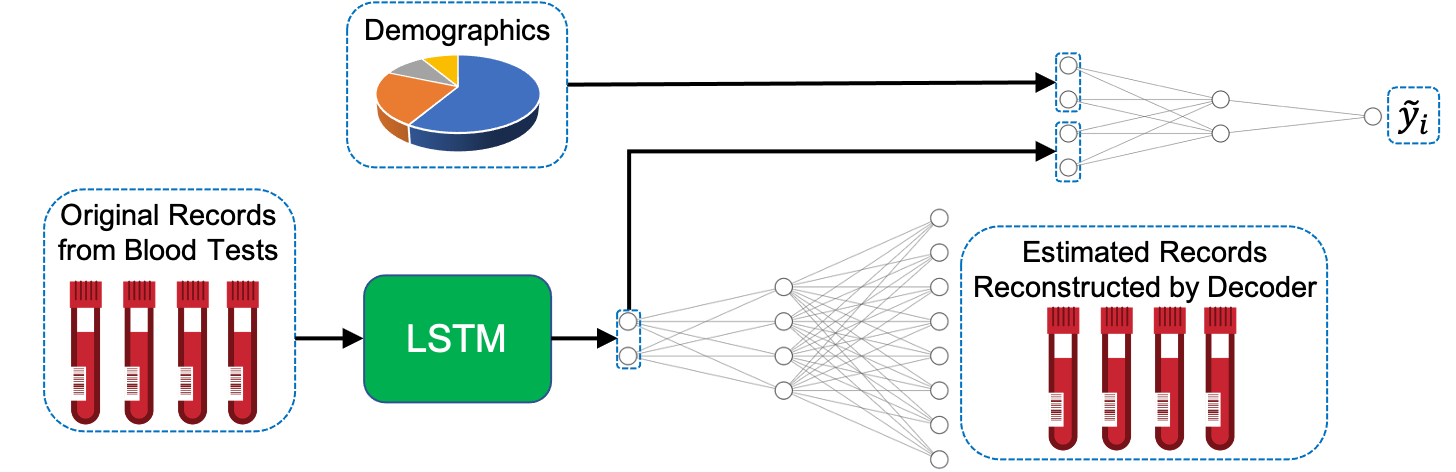
\includegraphics[width=0.9\textwidth]{figures/network-structure.png}
    \caption{The structure of the enrichment learning model. The enriched representation of dynamic records is in a fixed-length vector format which can be readily integrated with the static data.
    % The prediction via enrichment. MTS with uneven time intervals and missing data is represented by the sparse matrix $\mathbf{X}_i$ of varying size. We first compress the matrix of MTS into the enriched representation in a fixed length vector format, and then predict target labels from the enriched vectorial representation.
    } \label{fig: network structure}
\end{figure*}

\subsection{Notations}
In this paper, we denote a vector as a bold lower case letter and a matrix as a bold upper case letter. 
% For the arbitrary matrix $\mathbf{X}$, $\mathbf{x}^r$, $\mathbf{x}_c$, $x^r_c$ denotes the $r$-th row, $c$-th column, an element of $r$-th row and $c$-th column respectively. 
We use $i$ and $j$ to index the $i$-th patient and the $j$-th record respectively. We describe the records of the $i$-th patient as $\mathcal{X}_i = \{\mathbf{x}_i^s, \mathbf{X}_i, \mathbf{M}_i, \mathbf{t}_i\}$ as follows:
\begin{itemize}
    \item $\mathbf{x}_i^s \in \Re^{D_s}$ is a vector of static data.
    \item $\mathbf{X}_i = [\mathbf{x}_i^1; \mathbf{x}_i^2; \cdots; \mathbf{x}_i^{n_i}] \in \Re^{n_i \times D_l}$ are the longitudinal records collected from the blood tests across $n_i$ time points. Here the number of available records $n_i$ varies over the patients.
    \item $\mathbf{M}_i = [\mathbf{m}_i^1; \mathbf{m}_i^2; \cdots; \mathbf{m}_i^{n_i}] \in \{0, 1\}^{n_i \times D_l}$ are binary masks of observabilities of longitudinal records $\mathbf{X}_i$, where 1 and 0 indicate the observed and unobserved entry respectively.
    \item $\mathbf{t}_i = [t_i^1; t_i^2; \cdots; t_i^{n_i}] \in \Re^{n_i}$ are the time stamps of $n_i$ records.
\end{itemize}
The missing entries in $\mathbf{X}_i$ are initialized with the constant $0$. The target label $\mathbf{y}_i \in \{0, 1\}^{D_y}$ is the mortality of the $i$-th patient, which is provided in the training process if that patient is in the training set, such that $i \in \Omega$.

\subsection{Encoder}
We leverage the LSTM encoder $\phi_{E}: \Re^{n_i \times (2 D_l + 1)} \mapsto \Re^{d_z}$ to summarize longitudinal records and learn the temporal relationships between records. The time stamp of each record is crucial in learning the temporal relation between records (e.g. temporal locality) especially when the time intervals between the records are uneven. The pattern of missing entries helps the encoder to correctly interpret the input data. Thus, we provide the concatenation of longitudinal records, masks, and time stamps, $[\mathbf{X}_i, \mathbf{M}_i, \mathbf{t}_i] = [\hat{\mathbf{x}}_i^1; \hat{\mathbf{x}}_i^2; \cdots; \hat{\mathbf{x}}_i^{n_i}] = \hat{\mathbf{X}}_i \in \Re^{n_i \times (2 D_l + 1)}$, as an input of the LSTM encoder such that $\phi_{E}(\mathbf{X}_i, \mathbf{M}_i, \mathbf{t}_i;\ \theta_E) = \mathbf{z}_i$. Here, $\theta_E$ denotes the set of trainable parameters of the LSTM.

For each time step ($1 \leq j \leq n_i$), the input record $\hat{\mathbf{x}}_i^j$ of the $i$-th patient is processed by following the LSTM architecture~\cite{yu2019review}:
\begin{equation}
    \mathbf{k}^j_i = \sigma(\hat{\mathbf{x}}^j_i \mathbf{W}_{xk} + \mathbf{h}_i^{j-1} \mathbf{W}_{hk} + \mathbf{c}_i^{j-1} \mathbf{W}_{ck} + \mathbf{b}_k),
\end{equation}
\begin{equation}
    \mathbf{f}^j_i = \sigma(\hat{\mathbf{x}}^j_i \mathbf{W}_{xf} + \mathbf{h}^{j-1}_i \mathbf{W}_{hf} + \mathbf{c}^{j-1}_i \mathbf{W}_{cf} + \mathbf{b}_f),
\end{equation}
\begin{equation}\label{eq: cell state}
    \mathbf{c}^j_i = \mathbf{f}^j_i \odot \mathbf{c}^{j-1}_i + \mathbf{k}^j_i \odot \operatorname{tanh}(\hat{\mathbf{x}}_i^j \mathbf{W}_{xc} + \mathbf{h}^{j - 1}_i \mathbf{W}_{hc} + \mathbf{b}_c),
\end{equation}
\begin{equation}
    \mathbf{o}^j_i = \sigma(\hat{\mathbf{x}}_i^j \mathbf{W}_{xo} + \mathbf{h}^{j-1}_i \mathbf{W}_{ho} + \mathbf{c}^j_i \mathbf{W}_{co} + \mathbf{b}_o),
\end{equation}
\begin{equation}
    \mathbf{h}^j_i = \mathbf{o}^j_i \odot \operatorname{tanh}(\mathbf{c}^j_i),
\end{equation}
where $\sigma$ and tanh are the logistic sigmoid and hyperbolic tangent activation function respectively and $\mathbf{k}^j_i$, $\mathbf{o}^j_i$, $\mathbf{f}^j_i$ are the input, output, and forget gate of the $j$-th time step respectively. \{$\mathbf{W}_{xk}$, $\mathbf{W}_{hk}$, $\mathbf{W}_{ck}$, $\mathbf{W}_{xf}$, $\mathbf{W}_{hf}$, $\mathbf{W}_{cf}$, $\mathbf{W}_{xc}$, $\mathbf{W}_{hc}$, $\mathbf{W}_{xo}$, $\mathbf{W}_{ho}$, $\mathbf{W}_{co}$\} $\subset \mathbf{\theta}_E$ are trainable weight matrices and $\{\mathbf{b}_k, \mathbf{b}_f, \mathbf{b}_c, \mathbf{b}_o\} \subset \mathbf{\theta}_E$ are trainable bias vectors while $\mathbf{c}_i^j$ and $\mathbf{h}_i^j$ denote the cell state and hidden representation at the $j$-th time step. The hidden representation $\mathbf{h}_i^{n_i}$ at the last time step $n_i$ is our enriched representation of the longitudinal records $\hat{\mathbf{X}}_i$, such that $\mathbf{h}_i^{n_i} = \mathbf{z}_i \in \Re^{d_z}$.
\begin{equation}
    \phi_E(\mathbf{X}_i, \mathbf{M}_i, \mathbf{t}_i; \mathbf{\theta}_E) = \mathbf{h}_i^{n_i} = \mathbf{z}_i.
\end{equation}
Since the hidden representation at the $j$-th time point aims to summarize the records between the first and $j$-th time steps, the LSTM cell refers to the cell state $\mathbf{c}_i^j$ and reflects past records to $\mathbf{h}_i^j$. In Eq.~\eqref{eq: cell state} the cell state $\mathbf{c}_i^j$ is guided by the input gate $\mathbf{k}_i^j$ and forget gate $\mathbf{f}_i^j$, which control how much information should be preserved from the previous step, thus cell state $\mathbf{c}_i^j$ enables the hidden representation $\mathbf{h}_i^j$ to learn long term dependencies. For example, the input gate $\mathbf{k}_i^j$ and forget gate $\mathbf{f}_i^j$ can utilize the time stamp of each record to decide how much the hidden representation $\mathbf{h}_i^j$ should be updated. Therefore our encoder preserves the temporal locality of records with uneven time intervals while capturing the long term trends of a patient's status.
% For example, the LSTM encoder can capture the long term trends of a patient's status from the consecutive records.

% \subsubsection{Autoencoder}
% The encoder $\phi: \Re^{n_i \times (2 D_l + 1)} \mapsto \Re^{D_z}$ maps the input MTS in the high dimensional space into the latent representation in the lower dimensional space, such that $\phi_E(\mathbf{X}_i, \mathbf{M}_i, \mathbf{t}_i; \mathbf{\theta}_E) = \mathbf{z}_i \in \Re^{D_z}$. From the enriched representation $\mathbf{z}_i$, decoder $\phi_D: \Re^{D_z + 1} \mapsto \Re^{D_l}$ reconstructs the original record $\phi_D(\mathbf{z}_i ,t_i^j; \mathbf{\theta}_D) = \tilde{\mathbf{x}}_i^j \in \Re^{D_l}$, for each time point $t_i^j$ ($1 \leq j \leq n_i$). The predictor $\phi_P: \Re^{D_z + D_s} \mapsto [0, 1]$ generates the prediction $\phi_P(\mathbf{z}_i, \mathbf{x}_i^s; \mathbf{\theta}_P) = \tilde{y}_i$. $D_s, D_l, D_z$ denote the dimensionality of static, longitudinal, enriched biomarkers, and $\mathbf{\theta}_E, \mathbf{\theta}_D, \mathbf{\theta}_P$ denote the trainable parameters of encoder, decoder, predictor, respectively. 
% % Then we combine encoder, decoder, and predictor as a composite model, illustrated in Fig.~\ref{fig: autoencoder}.

% \subsection{Encoder}
% We leverage an LSTM encoder to compress MTS and extract long term dependencies in the temporal trend. 
% \subsubsection{Input}
% Because the time stamp of each record is crucial to learn the temporal trend and missingness pattern of the entries may represent the state of patient, we provide the concatenation of longitudinal records, masks, and time stamps $[\mathbf{X}_i, \mathbf{M}_i, \mathbf{t}_i] = \hat{\mathbf{X}}_i = [\hat{\mathbf{x}}_i^1; \hat{\mathbf{x}}_i^2; \cdots; \hat{\mathbf{x}}_i^{n_i}] \in \Re^{n_i \times (2 D_l + 1)}$ to the input layer of LSTM encoder. 
% The inputs of LSTM are $\hat{\mathbf{x}}_i^j$, $\mathbf{h}_{j - 1}$, $\mathbf{c}_{j - 1}$ and outputs are $\mathbf{h}_{j}$ and $\mathbf{c}_{j}$, where $\mathbf{h}_{j}$ is the hidden representation of records and $\mathbf{c}_{j}$ is the cell state of LSTM cell at $j$-th time step. 

% \subsubsection{Output}
% For each time step ($1 \leq j \leq n_i$), the input record $\hat{\mathbf{x}}_i^j$ of $i$-th patient is processed by following the LSTM architecture~\cite{yu2019review}:
% % The hidden representation $\mathbf{h}_j$ should compress the longitudinal records from first time step to $j$-th time step to accurately reconstruct the records, and the final hidden representation $\mathbf{h}_{n_i} = \mathbf{z}_i$ is the encoded representation of longitudinal records.
% \begin{equation}
%     \mathbf{k}^j_i = \sigma(\hat{\mathbf{x}}^j_i \mathbf{W}_{xk} + \mathbf{h}_i^{j-1} \mathbf{W}_{hk} + \mathbf{c}_i^{j-1} \mathbf{W}_{ck} + \mathbf{b}_k),
% \end{equation}
% \begin{equation}
%     \mathbf{f}^j_i = \sigma(\hat{\mathbf{x}}^j_i \mathbf{W}_{xf} + \mathbf{h}^{j-1}_i \mathbf{W}_{hf} + \mathbf{c}^{j-1}_i \mathbf{W}_{cf} + \mathbf{b}_f),
% \end{equation}
% \begin{equation}
%     \mathbf{c}^j_i = \mathbf{f}^j_i \odot \mathbf{c}^{j-1}_i + \mathbf{k}^j_i \odot \operatorname{tanh}(\hat{\mathbf{x}}_i^j \mathbf{W}_{xc} + \mathbf{h}^{j - 1}_i \mathbf{W}_{hc} + \mathbf{b}_c),
% \end{equation}
% \begin{equation}
%     \mathbf{o}^j_i = \sigma(\hat{\mathbf{x}}_i^j \mathbf{W}_{xo} + \mathbf{h}^{j-1}_i \mathbf{W}_{ho} + \mathbf{c}^j_i \mathbf{W}_{co} + \mathbf{b}_o),
% \end{equation}
% \begin{equation}
%     \mathbf{h}^j_i = \mathbf{o}^j_i \odot \operatorname{tanh}(\mathbf{c}^j_i),
% \end{equation}
% where $\sigma$ is logistic sigmoid activation function and $\mathbf{k}^j_i$, $\mathbf{o}^j_i$, $\mathbf{f}^j_i$ are input, output, forget gate of $j$-th time step respectively. \{$\mathbf{W}_{xk}$, $\mathbf{W}_{hk}$, $\mathbf{W}_{ck}$, $\mathbf{W}_{xf}$, $\mathbf{W}_{hf}$, $\mathbf{W}_{cf}$, $\mathbf{W}_{xc}$, $\mathbf{W}_{hc}$, $\mathbf{W}_{xo}$, $\mathbf{W}_{ho}$, $\mathbf{W}_{co}$\} $\subset \mathbf{\theta}_{E}$ are trainable weights matrix and $\{\mathbf{b}_k, \mathbf{b}_f, \mathbf{b}_c, \mathbf{b}_o\} \subset \mathbf{\theta}_{E}$ are trainable bias vectors. $\mathbf{c}_i^j$ and $\mathbf{h}_i^j$ denote the cell state and hidden representation. 

% In order decoder and predictor to reconstruct the original record and predict the target label accurately, the enriched representation should contain enough information for reconstruction and prediction, such as temporal trend of input sequence. The goal of encoder at $j$-th time pont is to generate the hidden representation $\mathbf{h}_i^j$ summarizing the records from first time step to $j$-th time step, therefore the LSTM cell refers to the cell state $\mathbf{c}_i^j$ and reflect the past records to $\mathbf{h}_i^j$. Since the cell state $\mathbf{c}_i^j$ is guided by the input gate $\mathbf{k}_i^j$ and forget gate $\mathbf{f}_i^j$ which control how much information came from previous step should be preserved, the cell state $\mathbf{c}_i^j$ enables the hidden representation $\mathbf{h}_i^j$ to learn the long term dependencies. For example, if the differences in the records and time intervals between the time points of recent 10 consecutive records are small, the hidden representation of 10 time steps before can be preserved.
% % and  and  Because input gate $\mathbf{k}_i^j$ and forget gate $\mathbf{f}_i^j$ control how much we keep the information came from previous step, therefore LSTM is able to convey the most useful inf
% The hidden representation $\mathbf{h}_i^{n_i}$ at the most recent time point is the enriched representation $\mathbf{z}_i$ of whole longitudinal records of $i$-th patent:
% % Then the enriched representation $\mathbf{z}_i$ is given to the decoder and predictor.
% \begin{equation}
%     \mathbf{h}_i^{n_i} = \mathbf{z}_i = \phi_E(\mathbf{X}_i, \mathbf{M}_i, \mathbf{t}_i; \mathbf{\theta}_E).
% \end{equation}

\subsection{Decoder}
From the enriched representation $\mathbf{z}_i$ of the longitudinal records, the decoder reconstructs the original record. We propose a decoder for dynamic data enrichment with a fully connected layers (FCL) architecture instead of another LSTM. Previous studies~\cite{srivastava2015unsupervised,sagheer2019unsupervised,saumya2020spam} that attempted to enrich longitudinal records with a recurrent neural network (RNN)~\cite{medsker2001recurrent}, did so by using RNNs for both the encoder and decoder, where the output (reconstructed record) of the decoder at each time step depends on the output at the previous time step. However, since no additional information is provided to the decoder other than a learned representation that is no longer longitudinal, there should not be a dependency between the outputs of the decoder. The enriched representation $\mathbf{z}_i$ summarizes \emph{whole} longitudinal records, thus decoder $\phi_D:\Re^{d_z + 1} \mapsto \Re^{D_l}$ should be able to reconstruct the $j$-th record $\mathbf{x}_i^j$ given the time stamp $t_i^j$ without any additional information, such that $\phi_D(\mathbf{z}_i, t^j_i;\ \theta_D) = \tilde{\mathbf{x}}_i^j \approx \mathbf{x}_i^j$, where $\theta_D$ is a set of weight matrices and bias vectors of the decoder. 
% This autoencoder architecture, to the best of our knowledge, has not yet been proposed. 

FCL consist of consecutive hidden layers as follows:
\begin{equation}
    \mathbf{h}_k = \sigma(\mathbf{h}_{k-1} \mathbf{W}_k + \mathbf{b}_k),
\end{equation}
where $\mathbf{h}_k$ is the output of the $k$-th hidden layer, $\sigma$ is the activation function, and $\mathbf{W}_k$, $\mathbf{b}_k$ are the trainable weights matrix and bias vector of the $k$-th hidden layer. To recover the original record at the specific time point, the decoder needs to know that time point. Thus the input vector of the decoder is the concatenation of the enriched representation $\mathbf{z}_i$ and the time stamp $t^j_i$, which is $[\mathbf{z}_i, t_i^j] \in \Re^{d_z + 1}$.  By forwarding the input to the decoder's FCL, we can generate the reconstructed record $\phi_D(\mathbf{z}_i, t_i^j; \mathbf{\theta}_D) = \tilde{\mathbf{x}}_i^j$, and we have the stack of reconstructed records of the $i$-th participant:
\begin{equation}
    \tilde{\mathbf{X}}_i = [\tilde{\mathbf{x}}_i^1; \tilde{\mathbf{x}}_i^2; \cdots; \tilde{\mathbf{x}}_i^{n_i}].
\end{equation}

\subsection{Prediction}
Because the learned representation of the dynamic data is in a fixed-length vector format, conventional classifiers can be connected to predict the target label. Because static data such as age may be crucial to predicting the target label, we provide the static data $\mathbf{x}_i^s$ with the learned representation $\mathbf{z}_i$ as an input $\mathbf{x}_i^P = [\mathbf{z}_i, \mathbf{x}_i^s] \in \Re^{d_z + D_s}$ of classifier $\phi_P$:
% which is $[\mathbf{z}_i, \mathbf{x}_i^s] \in \Re^{d_z + D_s}$. 
% By forwarding each input of the decoder and classifier to their own FCL, we can generate the reconstructed record $\tilde{\mathbf{x}}_i^j$ and prediction $\tilde{y}_i$ on the target label:
% \begin{equation}
%     \phi_D(\mathbf{z}_i, t_i^j; \mathbf{\theta}_D) = \tilde{\mathbf{x}}_i^j,
% \end{equation}
\begin{equation}
    \phi_P(\mathbf{z}_i, \mathbf{x}_i^s; \mathbf{\theta}_P) = \tilde{\mathbf{y}}_i.
\end{equation}
In this study we have chosen a Support Vector Machine (SVM) or FCL as a classifier. The support vector machine~\cite{vapnik1998support} leverages a kernel matrix to learn the nonlinear relationship between input and output. However, a medical dataset typically consists of many samples and computing the kernel matrix requires large resources. In addition, all the enriched representations must be prepared in advance to calculate the kernel matrix during the optimization process. Our semi-supervised learning model aims to optimize the prediction error and reconstruction error simultaneously for each batch of inputs. To tackle this problem, the previous study~\cite{rahimi2007random} proposed the random features mapping $\phi_F: \Re^{d_z + D_s} \mapsto \Re^{d_f}$ which approximates shift-invariant kernels efficiently. The SVM classifier first applies non-linear transformation $\phi_F: \Re^{d_z + D_s} \mapsto \Re^{d_f}$ to the enriched representation and then trains the linear model on top of the transformed features:
% SVM classifier consists of feature maps $\phi_F: \Re^{d_z + D_s} \mapsto \Re^{d_f}$ and linear mapping:
\begin{equation}
    \phi_F(\mathbf{x}_i^P) \mathbf{W}_{P} + \mathbf{b}_P = \tilde{\mathbf{y}}_i,
\end{equation}
where $\mathbf{W}_{P},\ \mathbf{b}_{P} \in \theta_P$ are the weights matrix and biases vector for the linear mapping from random feature to prediction.
\begin{figure*}[t]
    \centering
    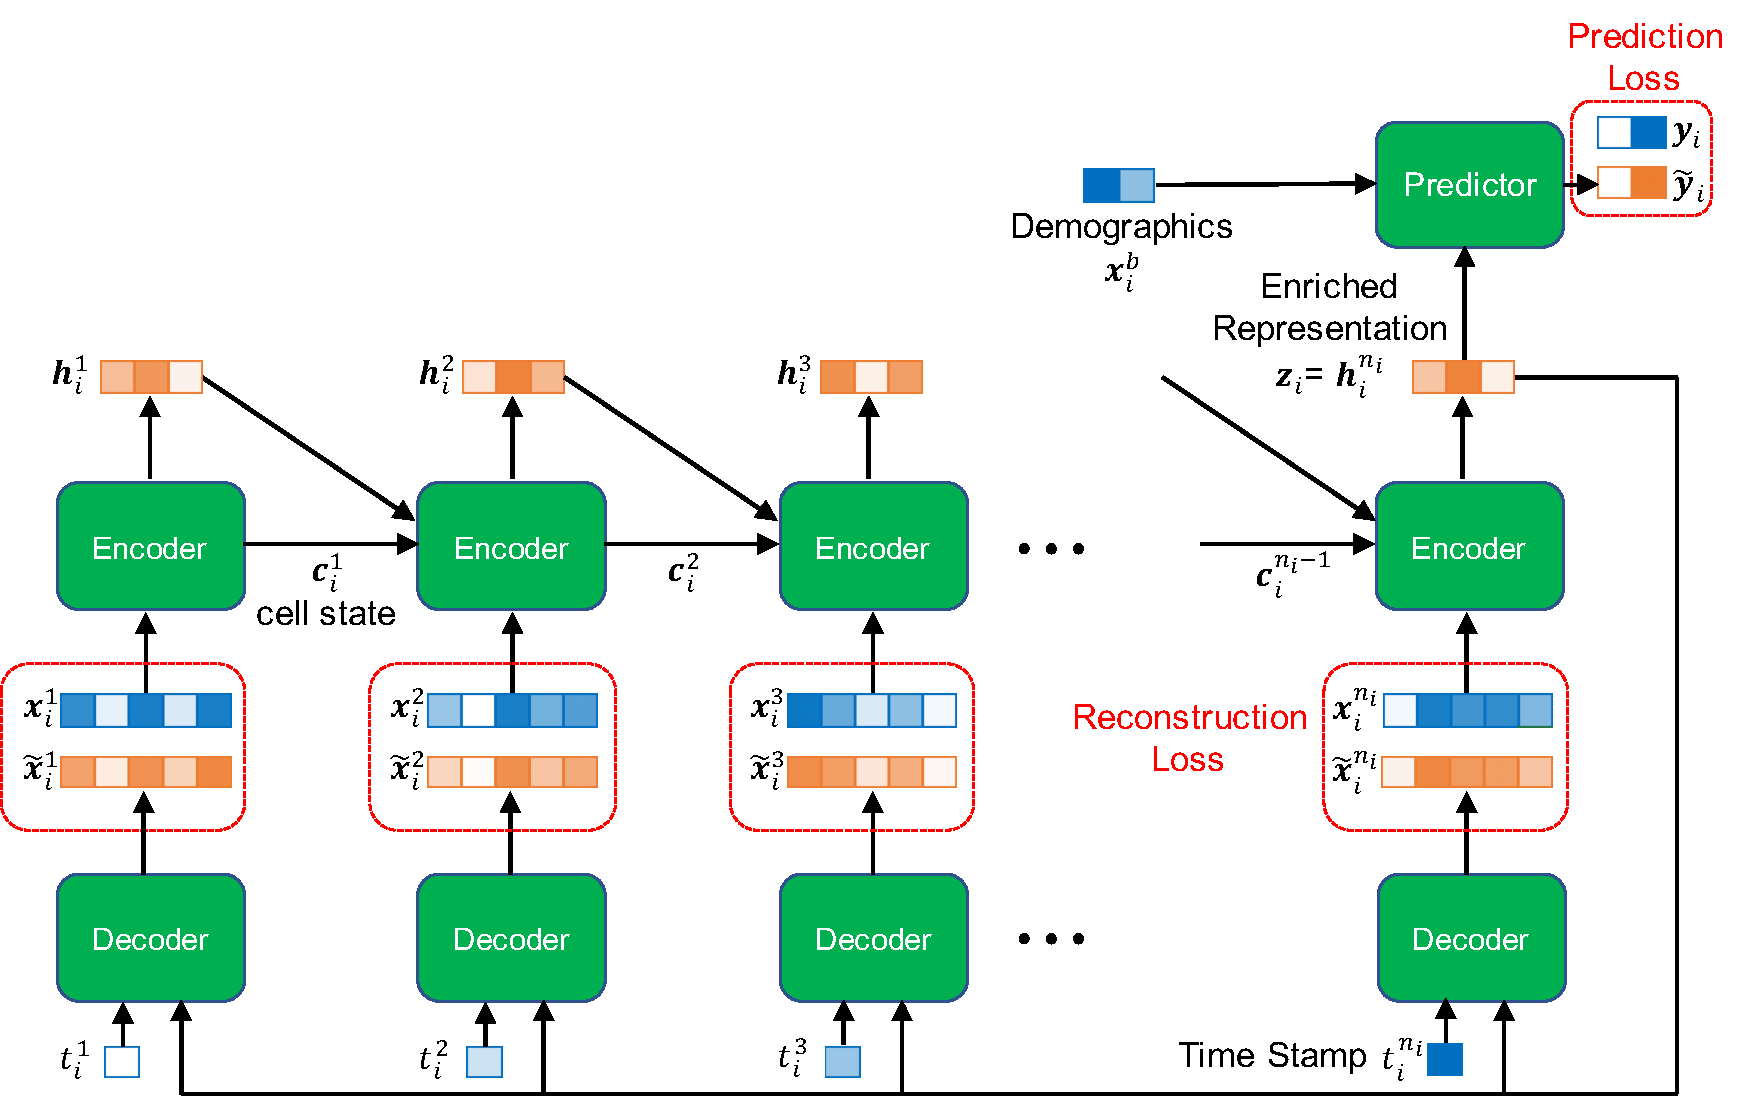
\includegraphics[width=0.8\textwidth]{figures/autoencoder.pdf}
    \caption{An illustration for the loss functions. The encoder consists of LSTM cells, which process the input record $\mathbf{x}_i^j$, and then generate the hidden representation $\mathbf{h}_i^j$ while conveying the cell state $\mathbf{c}_i^j$ to the next step. The enriched representation of the whole time series is defined as the hidden representation $\mathbf{h}_i^{n_i}$ at the last step.} \label{fig: autoencoder}
\end{figure*}
% \begin{equation}
%     \mathbf{\tilde{x}}_i^j = \sigma(\mathbf{W}_3 \sigma(\mathbf{W}_2 \sigma(\mathbf{W}_1 [\mathbf{z}_i, t_i^j] + \mathbf{b}_1) + \mathbf{b}_2) + \mathbf{b}_3) \sigma(\mathbf{W}_k\mathbf{h}_{k-1} + \mathbf{b}_k)
% \end{equation}
% In other words, the decoder should be able to reconstruct the original record with enriched vectorial representation $\mathbf{z}_i$ and time stamp $t_i^j$ if $\mathbf{z}_i$ successfully summarizes the records of all time steps. 

\subsection{Loss Functions}
The Semi-supervised autoencoder accomplishes two tasks: reconstructing the original records and predicting the target label by minimizing:
\begin{equation}\label{eq: objective}
    \min_{\theta_E, \theta_D, \theta_P} \mathcal{L}_{total} = \min_{\theta_E, \theta_D, \theta_P}(\gamma_1\mathcal{L}_{reconstruct} + \gamma_2\mathcal{L}_{predict}),
\end{equation}
where $\gamma_1$ and $\gamma_2$ are the hyperparameters to adjust the impact of each loss.
The reconstruction loss is defined as the scaled Mean Squared Error (MSE):
\begin{equation}
    \mathcal{L}_{reconstruct} = \frac{\left\| (\tilde{\mathbf{X}}_i - \mathbf{X}_i) \odot \mathbf{M}_i \right\|_F^2}{|\mathbf{M}_i|},
\end{equation}
where squared Frobenious norm $\| \cdot \|_F^2$ is defined as the summation of all the entries squared.

The prediction loss is defined with respect to the labeled $i \in \Omega$ and unlabeled $i \not\in \Omega$ data separately:
\begin{equation}
    \mathcal{L}_{predict} = \left\{\begin{array}{lr}
        - \alpha_c H(\tilde{{\mathbf{y}_i}}, \mathbf{y}_i), & \text{for } i \in \Omega\\
        0, & \text{for } i \not\in \Omega
    \end{array}\right\}.
\end{equation}
For the FCL predictor, $H(\tilde{{\mathbf{y}_i}}, \mathbf{y}_i)$ is defined as binary cross-entropy loss $\left\|\mathbf{y}_i \odot \operatorname{log}(\tilde{\mathbf{y}}_i) + (\mathbf{1} - \mathbf{y}_i) \odot \operatorname{log}(\mathbf{1} - \tilde{\mathbf{y}}_i)\right\|_1$ and $\mathbf{1}$ is a vector of 1's and $\operatorname{log}$ is an element-wise logarithm function. For the SVM predictor, $H(\tilde{{\mathbf{y}_i}}, \mathbf{y}_i)$ is defined as squared Hinge loss $(\operatorname{max}(1 - \mathbf{y}_i \cdot \tilde{\mathbf{y}}_i^T), 0)^2$.
%  where $\mathbf{y}_i, \tilde{\mathbf{y}} \in [-1, 1]^{D_y}$. 

Here we introduce the weighing factor $\alpha_c \in [0, 1]$ to alleviate the unbalanced distribution of labels when $c$ is the class of $\mathbf{y}_i$. For the unbalanced dataset, the target label has more observations in one specific class (majority class) than others (minority classes) and the prediction model may tend to classify most instances as the majority class to minimize the prediction error. To tackle this problem, we increase the prediction error for the minority classes by defining $\alpha_c = 1 - \frac{|\{j \in \mathbb{N}| y_j = c,\ j \leq N\}|}{N}$ for $N$ samples.


The high capacity unsupervised autoencoder may suffer from the tendency to learn trivial identity mapping and memorize the input~\cite{srivastava2015unsupervised} which is not useful for predicting the target label. However, the addition of our prediction loss function can prevent this memorization problem.

%Here the encoder LSTM is asked to come up with a state from which we can both predict the next few frames as well as reconstruct the input.
% This composite model tries to overcome the shortcomings that each model suffers on its own. A high-capacity autoencoder would suffer from the tendency to learn trivial representations that just memorize the inputs. However, this memorization is not useful at all for predicting the future. Therefore, the composite model cannot just memorize information.

% $L_{pred}$ is 0 when test set.
% Structure of LSTM, and if decoder is LSTM, then which state should be passed?
% Image for input (static + dynamic concatenation) and output (RE\_DATE is concatenated), and prediction target.
% LSTM unit explanation with maybe Figure. Concatenate static features because they are helpful to learn enrichment.
% Figure : Balance, reconstruction error vs prediction error.
% Why decoder is not RNN? Think of what is input for encoder and decoder. Because there is no information is additionally provided, current prediction depends on previous prediction does not make sense. The enriched representation is the fixed-length vector which is not longitudinal records anymore.
\section{Experiment}
Experiment here.
\iffalse
We proposed models based on LSTMs that can learn good video representations.
First, given that the proposed machine learning method is purely data-driven, our model may vary if starting from different datasets. As more data become available, the whole procedure can easily be repeated to obtain more accurate models.
We does not assume any property about dataset.

In this paper, we considered the identification of COVID-19 cases from X-ray images and proposed a novel semi-supervised deep architecture that can distinguish between the three cases of Healthy, non-COVID pneumonia, COVID-19 infection based on the chest X-ray manifestation of these classes. The proposed methodology is comprised of two modules: 1) the Task-Based Feature Extraction Network (TFEN), and 2) the COVID-19 Identification Network (CIN). 
\fi
%%%%%%%%%%%%%%%%%%%%%%%%%%%%%%%%%%%%%%%%%%%%%%%%%%%%%%%%%%%%%%%%%%%%%%%%%%%%%%%%%%%
\section{Conclusion}
We propose a semi-supervised enrichment method based on a novel LSTM autoencoder that is clinicaly applicable and can make real-time automatic mortality predictions. The enriched representation of MTS data is in a fixed-length vector format and can be readily integrated with the static data. In our experiments and case studies, the proposed model shows state-of-the-art performance in predicting mortality as well as increased flexability in handeling labeled and unlabled data. Additionly, when combined with the perturbation based feature identification method, our model identifies the risk factors of mortality that are consistant with the findings of previous medical studies and predictive models. 
% Our model is purely data-driven, which means the prediction performance can be further improved with additional data. 
Since there is no assumption or limitation in the dataset property, this research proposes the general framework to fully utilize the MTS dataset, and other models stemming from our enrichment approach are able to perform different prediction tasks.
\clearpage

%% The file named.bst is a bibliography style file for BibTeX 0.99c
\bibliographystyle{named}
\bibliography{bibliography}

\end{document}

